\documentclass[12pt,twoside]{reedthesis}
\usepackage[hyphens]{url}
\usepackage{amsmath}
\usepackage{amssymb}
\usepackage{amsthm}
\usepackage{booktabs}
\usepackage{graphicx}
\usepackage{latexsym} 
\usepackage{longtable}
\usepackage{rotating}
\usepackage{setspace} 
\usepackage{xcolor} 
\usepackage{graphicx}
\graphicspath{ {./images/} }
%\usepackage{natbib}
%\usepackage[style=reading,backend=bibtex8]{biblatex} \addbibresource{bibliography.bib}
\setlength{\parskip}{0pt}
\newcommand{\red}[1]{\textcolor{red}{#1}}
\newcommand{\todo}{\red{TODO}}

\title{An Overview of Superoptimizers}
\author{Elijah Wheelock}
\date{May 2024}
\division{Mathematics and Natural Sciences}
\advisor{Greg Anderson}
\department{Computer Science}

\begin{document}

\maketitle
\frontmatter % this stuff will be roman-numbered
\pagestyle{empty} % this removes page numbers from the frontmatter
% \chapter*{Acknowledgements} % Acknowledgements are optional
% I'd like to thank Greg, Tobey, Jennifer, Arthur, Norman, and Susan.
% \chapter*{Preface} % The preface is optional
\tableofcontents

\chapter*{Abstract} % If your abstract is longer than a page, there may be a formatting issue.

% Reiterate in introduction
Superoptimization is a family of compilation techniques which seek to improve the characteristics of computer programs by computational (non-heuristic) means.
This is seen as distinct from "ordinary" optimization (perhaps more properly called meliorization), which seeks to improve programs by application of a large number of rewrite rules.
Another view is that superoptimization recharacterizes the problem of program improvement as a search problem, rather than an equational reasoning problem.
More broadly, superoptimization may be seen as an application of the techniques of program synthesis to the domain of concretely-realized (assembly code/IR) programs.
In practice, there is an infinite number of potential programs which compute the desired result, many of which are intuitively non-obvious.
Therefore it is desirable to have special techniques for synthesizing (generating), pruning, and verifying such candidate programs. 
In this paper, we will survey a variety of methods from the literature that have been used for these ends.

% \chapter*{Dedication}
\mainmatter % here the regular arabic numbering starts
\pagestyle{fancyplain} % turns page numbering back on
\chapter*{Introduction} % The \introduction command is provided as a convenience. % if you want special chapter formatting, you'll probably want to avoid using it altogether
    \addcontentsline{toc}{chapter}{Introduction} % intro gets included in the table of contents
    \chaptermark{Introduction}
    \markboth{Introduction}{Introduction} % make sure that the headers are right. % don't number intro as 1 so that chapter one is 1.
    \singlespacing % \onehalfspacing % \doublespacing

% cite some stuff! E.g. Turing on undecidability
% probably anything a CS senior wouldn't know should be cited

Since the introduction of the term by \cite{massalin1987superoptimizer}, a wide variety of techniques have been harnessed to the goal of superoptimization.
These techniques may be broadly categorized in several ways, including:
    the goals (optimization criteria) of the superoptimization system,
    the techniques used for synthesis and/or verification of generated programs,
    the problem domain,
    and the capabilities/limitations of the system.
In this paper we will focus on categorizing systems by synthesis technique, but first it seems advisable to briefly cover the other possible taxonomies.

In writing any kind of optimizer, one must first select a criterion by which to rank candidate programs.
There are a few potential measures by which to do so.
Perhaps the most immediately salient is performance: 
    in almost every application, faster programs are preferred to slower ones.
Another common goal is to reduce resource use: 
    for example, a program which needs less memory is preferable to one which uses more.
There are also other resources whose conservation might be desired, for example 
    functional units on an FPGA, 
    power or space on a hardware design, 
    disk writes, 
    or disk or network bandwidth.
A less-common goal is to reduce the code size of generated programs.
    This might be desired for 
        performance reasons (reducing instruction cache misses or instruction pipeline delays), 
        or because the output code is meant to run on a resource-poor system such as a microcontroller, 
        or for entertainment ("code golfing").

% Motivation: We want to improve these criteria! superoptimization is one way to do that!
All these criteria represent possible desiderata in modifying our programs.
That is to say, these criteria are also the motivations behind writing optimizers and superoptimizers. 
\red{TODO} %FIXME

Another possible taxonomy is by problem domain.
Many superoptimizers focus on assembly programs with integer operands, because there are powerful techniques for verifying such programs, but by no means all.
There have also been interesting superoptimizers targeting 
    floating-point assembly programs, 
    compiler intermediate representation (IR) programs, 
    and high-level synthesis (HLS) languages for integrated circuit (IC) or field-programmable gate array (FPGA) development.

A related way to categorize superoptimizers is by the limits they set on their problem domain.
For example, a common limitation is that the output code must be expressible in a loop-free way
    -- loops are a difficult problem for many approaches,
        not least because verifying equivalence of programs with loops is in general undecidable,
        and because heuristic testing of loops may require unbounded time.
Another common problem in superoptimizers is that it's very difficult to produce an accurate cost estimation for memory access.
    Modern computer systems generally have many-layered information storage systems, with multiple layers of caching, batching, and indirection between them, making the estimation of latency for any particular memory access very difficult.
    For this reason, black-box measurement of performance is the gold standard, but this is sometimes cost-prohibitive.
Finally, the overall difficulty of any search problem scales with the size of the search space, which in superoptimization scales exponentially with the length of the synthesized program.
    Therefore most superoptimization systems are limited mainly by available computation power, and impose a maximum synthesized program size for performance reasons.

\red{TODO} talk about difficulties synthesizing constants, memory access, %TODO 

There are also multiple approaches for verification of synthesized programs.
Perhaps the simplest is heuristic testing: 
    directly measuring the output of the synthesized program against a set of test cases, usually generated by the input (unoptimized) program.
Another approach is boolean verification: using a SAT solver to prove bitwise equivalence of the program's inputs and outputs.
This is potentially very expensive, but if done correctly guarantees the correctness of the generated program. 

\red{TODO}

Most interestingly for our purposes, superoptimizers can be categorized by the approach they take to synthesis of superoptimized programs.
This is the measure on which published systems vary most widely, and the selection of approach is perhaps the most salient question for the authors of new systems.
These approaches vary widely in sophistication, complexity, and power.

Perhaps the simplest possible approach, pioneered by \cite{massalin1987superoptimizer}, is simple enumeration. 
The technique is to line up all possible programs in order of length, testing each in turn by the selected verification strategy. 

\red{TODO}: maybe explain about citations per-paper per-Subsubsection

%\begin{itemize}
%    \item intro: \cite{massalin:87}
%    \begin{itemize}
%        \item why superoptimization $\leftarrow$ I think I need more here
%        \item standard compilation (heuristic optimization)
%        \item search problem
%        \item wide variety of techniques: can categorize by
%        \begin{itemize}
%            \item goals of superoptimization
%                \begin{itemize}
%                    \item code size
%                    \item performance
%                    \item resource use
%                \end{itemize}
%            \item problem domain
%                \begin{itemize}
%                    \item assembly
%                    \item IR
%                    \item HLS: FPGA/hardware
%                \end{itemize}
%            \item capabilities
%                \begin{itemize}
%                    \item loops or loop-free
%                    \item memory access
%                    \item max code length
%                \end{itemize}
%            \item synthesis approach
%            \item verification approach
%        \end{itemize}
%    \end{itemize}
%    \item approaches to superoptimization
%    \begin{itemize}
%        \item (synthesis techniques vs verification techniques?)
%        \item enumeration % 2-09
%        \item logic/smt % 2-16
%        \item symbolic % 2-23
%        \item stochastic search
%        \item ml
%        \item other/multiple
%        \begin{itemize}
%            \item derive pre/post-conditions OR require formal eqv
%        \end{itemize}
%    \end{itemize}
%    \item capabilities
%    \begin{itemize}
%        \item code length
%        \item loops
%        \item domain
%        \item Superoptimization (software) vs High-level synthesis (hardware)
%    \end{itemize}
%\end{itemize}

\chapter{Beginnings: Enumeration}
\red{TODO} merge into symbolic

\subsubsection{Superoptimizer -- A Look at the Smallest Program}
Happily, the earliest published superoptimizer is also among the simplest, and so will serve admirably as an introduction to the idea. 
The word "superoptimizer" dates from Henry Massalin's paper, "Superoptimizer -- A Look at the Smallest Program" \cite{massalin1987superoptimizer}.
Massalin's superoptimizer, like most superoptimizers, operates in three main phases: synthesis, pruning (optional), and verification.

The synthesis stage in this system is, perhaps, the simplest imaginable: simply write down all assembly programs in alphabetical order.
The advantage of this approach is that if a result is found, it will be the smallest possible code that can compute the desired result, and therefore likely relatively fast as well;
the disadvantage is that the search space blows up exponentially with the length of function sought, making it intractable for all but the smallest code segments.

The pruning stage is also relatively simple. There are some obviously-spurious code sequences if what is sought is the shortest possible correct code, e.g. "move X,Y; move Y,X".
Code containing such sequences may be rejected early, before the more-expensive verification stage.

Massalin gives two distinct approaches to verification, driven by resource limitations.
The reliable, but slow and expensive way, is to logically test the bitwise equivalency of the candidate program to the desired program, using what Massalin calls a "boolean program verifier".
As we'll see soon, this approach has become much more practical in the years since then, due to improvements both in hardware and SMT solvers. 
%TODO %FIXME

This system, although relatively simple, and harshly limited by the available computation hardware of its era, achieves some interesting results -- \red{TODO} %FIXME

\subsubsection{Automatic Generation of Peephole Superoptimizers}

One clever way to reduce the expense and inconvenience associated with running a superoptimizer to improve your code is to precompute it
-- that is, to cache the results of superoptimizing common code segments, and use these results as part of the peephole stage of an ordinary optimizer.
Such is the strategy adopted by Bansal and Aiken \cite{bansal2006peephole}.

%FIXME
This system works by harvesting code segments from a large corpus of existing programs, with certain restrictions, and superoptimizing them. 
In contrast to Massalin's superoptimizer, it uses a runtime-estimate based cost function, as opposed to length-based.

The selection of code segments is somewhat involved.
One problem that might occur with superoptimizing a code segment is that it might disturb invariants relied on by other parts of the program.
When the code segment is selected manually, this is not a problem.
But for automatic selection, the system has to be confident that the segments won't be jumped into from elsewhere. 

It also uses a different pruning strategy.
Before testing an instruction sequence, it is first canonicalized by renaming the registers it uses in a consistent way.
If the canonicalized form has already been checked, then the sequence may be safely pruned.

The verification strategy is similar to Massalin's boolean verifier, but using a SAT solver.
This approach had become much more practicable in the intervening time between these publications due to algorithmic and hardware advances.

Bansal and Aiken's system achieves quite impressive results 
    -- a speedup by a factor of between 1.7 and 10, (mean ~4.9) in compute-intensive programs, with a 1-5\% speedup in more general programs, all compared to code nominally already optimized by the compiler.

\chapter{Symbolic Search}

\red{TODO:} Chapter intro: what is symbolic search?

\subsection{SMT}

\red{TODO}: add background, SAT solver, 

\subsubsection{Denali: A Goal-directed Superoptimizer}
This paper \cite{joshi2002denali} uses an automated theorem prover to simultaneously synthesize and verify new programs.
It takes a program in a custom low-level language, expresses it in a symbolic form as a graph of all equivalent ways of computing its output expressions called the E-graph, and formulates the conjecture that "no program of the target architecture computes the values of the goal terms within K cycles" as an input to a satisfiability solver. 

The graph re-writing uses a fairly standard term-rewriting strategy, with the addition of a notion of equivalence for graph nodes.
The connections between the E-graph nodes are then translated into clauses for the use of the SAT solver.

The satisfiability step requires a little more detail.
In order to logically express the number of cycles required for the whole program, it has to express the time by which every intermediate step will be completed.
To do this, Denali uses an additional set of constraints on the times of launching, completion, and availability, which may be roughly summarized by the following slogans:
    A computation is completed after its latency has elapsed since its launch time.
    A computation can't be launched until its arguments are available.
    A value is available at all times at or after its completion time.
    Only one operation may be launched per cycle (The paper gives some remarks on extending to multiprocessing systems, but does not explain in detail).

\red{TODO:} mapping of E-graph to SAT clause

\subsubsection{Unbounded Superoptimization}
Related to Denali is the work by Jangda and Yorsh in "Unbounded Superoptimization" \cite{jangda2017unbounded}.
Rather than matching E-graphs, which in the intervening years had been integrated into SMT solvers, it to directly encodes the target program as a logical formula.
It does this by encoding the input program, treating it as the first candidate output, and "squeezing" it by imposing lower and lower cost bounds on the solver. This "top-down" approach has the advantage that if the superoptimizer is halted early, it can still return a correct output, unlike many superoptimizers which work "bottom-up" and thus start without any candidate programs.

\red{TODO} LLVM phi nodes?

\subsection{CEGIS}

\red{TODO}: CEGIS, usually goes with some kind of enumeration too
\red{TODO}: explain CEGIS (briefly-ish) (each counterexample rules out at least one program, so you mostly always make progress, usually quickly).

\subsubsection{Souper: A Synthesizing Superoptimizer}
Souper \cite{sasnauskas2017souper} is an engineering project to create a superoptimizer working on LLVM IR.
This is desirable because LLVM is used as the "middle end" for a large number of compiler projects, and therefore Souper can be used for a wide variety of languages and target architectures.
It has three main components:
    an extractor, to produce Souper IR from LLVM IR,
    a synthesizer using counterexample-guided interactive synthesis,
    and a verifier using an SMT solver.

\red{TODO}: cite Solar-Lezama et al. "Combinatorial Sketching for Finite Programs"
\red{TODO}: cite Gulwani et al. "Synthesis of loop-free programs"?

Souper uses a custom IR analogous to a purely-functional subset of LLVM IR without control flow\footnote{Some information about control flow external to the code section under consideration is preserved, but control flow operations within a code section are forbidden.}, represented for computational purposes as a directed acyclic dataflow graph.
It is also limited to integer instructions; it has no model for floating-point, memory, or vector operations.
The operands of programs in this IR are considered only as bitvectors (parameterized by width) or tuples of bitvectors.

\red{TODO:} a bit on the synthesizer

\red{TODO}: Threats to soundness:
    Souper bugs,
    LLVM bugs,
    Solver bugs,
    Undefined behavior: One issue with relying on the semantics of LLVM is that there are areas of undefined behavior!

\subsubsection{Dataflow-Based Pruning for Speeding up Superoptimization}
\red{TODO:} a little bit about why pruning holes early is desirable.

This paper \cite{mukherjee2020dataflow} enhances Souper with an additional family of pruning strategies based on dataflow reasoning. 
Pruning spurious candidates as early as possible is obviously highly desirable.
This paper uses both forward and backward dataflow analysis techniques to prove candidate expressions incorrect before they are fully substantiated (while they still contain "holes", constants or sub-expressions which have yet to be synthesized).
The forward techniques are known bits,
                           integer ranges, and
                           bivalent bits.
The backward techniques are required bits,
                            don't-care bits, and
                            forced bits.

\red{TODO:} put in examples, OK to use originals.

The known-bits analysis works by proving that certain bits of the output of the candidate program are necessarily incompatible with the specification.
For a simple example, if the specification ends by setting the rightmost bit of the output to 1, then any candidate which ends with a left shift can be immediately dismissed.
The integer ranges analysis is similar, but considering the magnitudes of outputs instead of their bits.
The bivalent-bits analysis extends known-bit analysis by proving that certain bits of the candidate are indeterminate while the corresponding bits of the input are known.

The required-bits analysis works by proving that certain bits of the input to the specification are \emph{required}, i.e. that changing its value can change the output. If such an input is not used in a candidate program, then that program can be safely pruned; e.g. if the specification is $x + y$, but the candidate is $x + C$ where $C$ is constant.
The forced-bits analysis is in a way analogous to the known-bits analysis, working in the opposite direction. It works by finding conflicts in candidates with symbolic (not-yet-synthesized) constants. Intuitively, it can be thought of as finding inconsistencies in a system of equations based on comparing the candidate to the specification. %rephrase?

\red{TODO:} Something about results

%Present CEGIS first, then decide if this is still in
% \subsubsection{From Relational Verification to SIMD Loop Synthesis}
% \cite{barthe2013simdloopsynth}

\chapter{Stochastic Search}
\red{TODO:} motivate chapter perhaps with weaknesses of previous approaches.

\subsubsection{Stochastic Superoptimization}
Heretofore we have limited ourselves to superoptimizers which operate in a deterministic regime.
However, there is another way to think of the problem: as an unguided search in a high-dimensional, irregular search space.
While this way of thinking loses some desirable properties from more deterministic approaches, such as guaranteed progress or "solutions" for small problems, it also unlocks a variety of techniques for use in superoptimization, which may scale better than deterministic techniques.

\red{TODO:} Explain MCMC a bit more clearly.

One such technique is markov chain monte carlo sampling, pioneered by \cite{schkufza2013stoke}. 
Essentially, the strategy works by drawing candidate rewrites from a distribution with favorable properties (in this case, a bias toward low cost).
The candidates are then scored by a cost function taking into account estimates of both and performance.
A candidate which scores better than the current best is always accepted; a worse one is accepted with probability proportional to $1/e^(c'/c)$, where $c$ is the cost of the old candidate and $c'$ is the cost of the new one.

\red{TODO:} 

\red{TODO:} Explain hamming distance. DONE

Correctness is estimated by the hamming distance (bitwise difference: the number of corresponding bits that differ between the two strings, plus insertions, if needed) between the outputs of the candidate and those of the specification.
Cost is estimated by the sum of the (average) latencies of the instructions in the candidate.

There are two phases to the search performed by \textsc{Stoke}:
    what they call synthesis, in which initially random programs are permuted to search for programs equivalent to the specification in disconnected parts of the search space,
    and optimization, in which correct programs are permuted in search of better performance.
The top 20\% of candidates are then formally verified and tested for performance, and the best candidate is returned.

\red{TODO}: Results and limitations

\subsubsection{Conditionally Correct Superoptimization}

One problem with the kind of bitwise verification accomplished by SMT solvers is that in some sense it's actually too exact.
This has the disadvantages both of added expense for verifying more than necessary, and in rejecting correct but inexactly equivalent candidate optimizations.
There are multiple reasons that successful optimizations might not be bitwise equivalent to the specification
    -- for example, the differences might only appear in a region of input space which is forbidden for some reason.
While there are a number of existing efforts to produce relaxation conditions from annotations given by the programmer to a traditional compiler, another possibility is to attempt to have the compiler generate them itself for review by the programmer.
Such is the project of \cite{sharma2015conditionally}.
    
This paper expands on \textsc{Stoke} with the intention of proving correctness more rigorously than the test-case based approach it originally used.
It does this by augmenting it with a new verification algorithm, which they call \textsc{Cove}.
This algorithm works using a formal verification system for x86 assembly created by the same authors \cite{sharma2013ddec} (modulo certain pointer aliasing changes) to generate verification conditions for the candidate program, which are then fed into \textsc{Cove} to produce a set of preconditions that make the target and candidate equivalent. These preconditions are then presented to the programmer, and if accepted, the candidate program is considered correct.
    
The aliasing changes mentioned above constitute a relaxation of the formal verification process -- it turns out that reasoning about aliasing is a relatively expensive part of the verifier, and that it is the grounds for rejection for a large number of candidates. Therefore, rather than considering every possible case of pointer aliasing, only those which are relevant in the traces for the given test cases are considered. This does not affect the overall correctness of \textsc{Cove}, since the derived non-aliasing assumptions are included (explicitly or implicitly) in the final set of preconditions presented to the user.
    
The preconditions are generated from the verification conditions via abstract interpretation by conjuncting abstractions of the test inputs on which the target and candidate are equivalent in progressively more-restrictive abstract domains. The domains used in \textsc{Cove} are bitvector alignment to 1, 2, 4, 8, 16, 32, and 64 bytes, bit-vector equalities, and bit-vector intervals (interpreted as intervals of unsigned integers).
    
\red{TODO:} ask Greg about what exactly the abstraction function is doing

\red{TODO:} a little background on abstract interpretation

\red{TODO:} a little about results

\subsubsection{Scaling up Superoptimization}

% cancelled: covered by \cite{phothilimthana2016scaling}
%\subsubsection{\textsc{GreenThumb:} Superoptimizer Construction Framework}
%\cite{phothilimthana2016greenthumb} %GreenThumb is a superoptimizer written for 

Perhaps it's a natural question, when comparing the strengths and weaknesses of various superoptimization techniques, to ask, "why not use them all together, and let the strengths of each cover the weaknesses of the others?"
Phothilimthana et al. attempt precisely this in \cite{phothilimthana2016scaling}.
They also spend considerable effort comparing and contrasting results achieved by various techniques.
    
This paper uses multiple techniques for synthesis in a "cooperative superoptimizer".
\textsc{Lens}, a new enumerative superoptimization algorithm,
a sliding-window strategy to decompose programs too large to superoptimize directly,
and a synthesizer combining communicating symbolic, stochastic, and enumerative search programs.
Verification is accomplished by an equivalence requirement in the pruning step.
    
\textsc{Lens} is an enumerative algorithm which uses a bi-directional (pre- and post-conditional) pruning strategy to cut down the search space.
It works by considering the space of programs to enumerate as composed of a set of equivalence classes of input-output behaviors on a reduced bitwidth, and attempting to bridge the gap between the input and the output of the specification.
If such a bridge is found, it is verified using a constraint solver; if accepted, it's returned, but if rejected, the constraint solver returns an input counterexample, which is then used as a test case to prune further candidates.

.he sliding window strategy is fairly simple; it randomly picks a window of the program to superoptimize, attempts to improve it, and repeats until no position of the window yields an improvement to the program.
There is one additional detail that bears mentioning: 
this window decomposition allows the verification step to use the context of the surrounding program when checking equivalence; rather than checking equivalence of the candidate with the target, it can check the equivalence of the sequence prefix-candidate-postfix with the sequence prefix-target-postfix.
This allows a few additional optimizations.

The strategies used in the "cooperative superoptimizer" are
    \textsc{Lens} on the whole program,
    \textsc{Lens} with window decomposition,
    an SMT solver on the whole program,
    an SMT solver with window decomposition,
    \textsc{Stoke} starting from a random program, and
    \textsc{Stoke} starting from the specification program.
The communication between synthesizers takes the form of a shared best solution, $p_{best}$.
The whole-program \textsc{Lens} and SMT synthesizers don't use $p_{best}$. The others restart their synthesis, using $p_{best}$ as the new starting point instead of the target.

Results: \red{TODO}

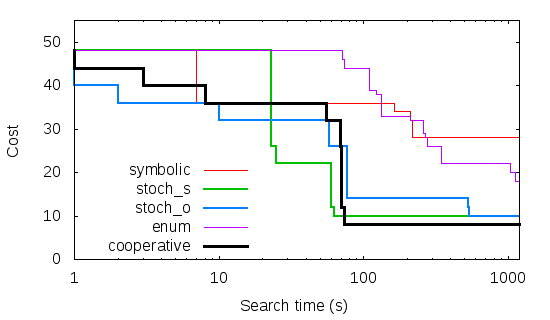
\includegraphics[scale=0.5]{scaling}

% on backburner
%\subsubsection{Sound Loop Superoptimization for Google Native Client}
%\cite{churchill2017soundloop}

%\subsubsection{Learning Performance-Improving Code Edits} \cite{}

\subsubsection{Learning to Superoptimize Programs}
\cite{bunel2017learning}
Augment \textsc{Stoke} by learning the proposal distribution.

\subsubsection{Deep Symbolic Superoptimization Without Human Knowledge}
\cite{hui2020deep}

\subsubsection{Learning to Superoptimize Real-World Programs}
\cite{shypula2022learning}

\chapter{Conclusion}

\red{TODO:} future work?, comparison of techniques, 

% briefly summarize intro, talk about different approaches again, advantages & disadvantages
% more results-focused
% if I've noticed open directions, point them out

%\appendix
%    \chapter{Appendix 1}

\backmatter
%\nocite{*} 
%\printbibliography
\bibliographystyle{apalike}
\bibliography{bibliography}
% To force capitalization in an article title or where all lowercase is generally used, bracket the capital letter in curly braces.
% optionally, an index would go here.

\end{document}
